\documentclass[12pt,a4paper]{article}

% Packages
\usepackage[utf8]{inputenc}
\usepackage{amsmath, amssymb}
\usepackage{graphicx}
\usepackage{hyperref}
\usepackage{listings}
\usepackage{color}
\usepackage{geometry}
\usepackage{caption}
\usepackage{fancyhdr}
\usepackage{url}
\usepackage{xspace}
\usepackage[backend=bibtex,style=alphabetic]{biblatex} % Use biblatex with the alphabetic style
\addbibresource{references.bib}

\geometry{a4paper, margin=1in}

% Header and Footer
\pagestyle{fancy}
\fancyhf{}
\fancyhead[L]{\leftmark}
\fancyhead[R]{\rightmark}
\fancyfoot[C]{\thepage}

% Listings settings
\definecolor{codegray}{gray}{0.9}
\lstset{
  backgroundcolor=\color{codegray},
  basicstyle=\ttfamily,
  numbers=left,
  numberstyle=\tiny,
  stepnumber=1,
  numbersep=5pt,
  tabsize=4,
  breaklines=true,
  breakatwhitespace=false,
  showspaces=false,
  showstringspaces=false
}

\newcommand{\Partition}{\textit{Partition}\xspace}
\newcommand{\Knapsack}{\textit{Knapsack}\xspace}
\newcommand{\SubsetSum}{\textit{Subset-Sum}\xspace}
\newcommand{\MultPart}{\textit{Multiway Partitioning}\xspace}
\newcommand{\tildeO}{\tilde{O}}
\newcommand{\ApxPartition}{\textit{Approximate Partition}\xspace}

\begin{document}

% Title Page
\begin{titlepage}
    \begin{center}
        \vspace*{1cm}
        
        \Huge
        \textbf{Title of Your Thesis}
        
        \vspace{0.5cm}
        \LARGE
        Subtitle (if any)
        
        \vspace{1.5cm}
        
        \textbf{Your Name}
        
        \vfill
        
        A thesis submitted in partial fulfillment of the requirements for the degree of\
        Bachelor of Science in Computer Science
        
        \vspace{0.8cm}
        
        
\includegraphics[width=0.4\textwidth]{university_logo.png}
        
        \Large
        University Name\
        Department Name\
        \today
        
    \end{center}
\end{titlepage}


% Sections
\section{Introduction}
\subsection{Problem Statements}
In it's simplest terms \Partition is the problem of selecting a subset of integers from a list such that the sum of the integers in the subset is as close as possible to half the sum of all the integers in the list. \Partition, due to its simple formulation, is a special case of the \MultPart, \SubsetSum, and in turn \Knapsack problems. 
Below are the formal statements of these problems and \Partition defined in terms of its generalisations.

\subsubsection{Reductions from \Knapsack}

\paragraph{\Knapsack Problem:}
In the Knapsack problem, the input is a list of \(n\) items \\ \((p_1, w_1), \ldots, (p_n, w_n) \in \mathbb{N} \times \mathbb{N}\) together with a knapsack capacity \(W \in \mathbb{N}\), and the optimal value is
\[
    \text{OPT} := \max_{J \subseteq [n]} \left\{ \sum_{j \in J} p_j \, \bigg| \, \sum_{j \in J} w_j \leq W \right\}.
\]

\paragraph{\textit{Subset-Sum} Problem:}
The \SubsetSum is a special case of the \Knapsack problem where the weights are equal to the profits, i.e., \(w_i = p_i\) for all \(i \in [n]\). For the input list of \(n\) integers \(x_1, \ldots, x_n \in \mathbb{N}\) and an integer \(W\), the optimal value is
\[
    \text{OPT} := \max_{J \subseteq [n]} \left\{ \sum_{j \in J} x_j \, \bigg| \, \sum_{j \in J} x_j \leq W \right\}.
\]

\paragraph{\Partition Problem:}
The \Partition problem is a special case of the \SubsetSum problem where \(W\) is half the sum of the integers in the input list. For the input list of \(n\) integers \(x_1, \ldots, x_n \in \mathbb{N}\), the optimal value is
\[
    \text{OPT} := \max_{J \subseteq [n]} \left\{ \sum_{j \in J} x_j \, \bigg| \, \sum_{j \in J} x_j \leq \frac{1}{2} \sum_{i \in [n]} x_i \right\}.
\]

\subsubsection{Reduction from \MultPart}
\paragraph{\MultPart Problem:}
The \MultPart problem is the problem of partitioning a list of \(n\) integers into \(k\) disjoint subsets such that the sum of the integers in each subset is as close as possible. The exact objective can be described in several ways:
\begin{itemize}
    \item Minimise the difference between the largest and the smallest of the sums.
    \item Minimise the largest sum, or equivalently, maximise the smallest sum.
\end{itemize}
Although there are not equivalent in the general case, for \Partition they are. We will use the former formulation.
Given a list of \(n\) integers \(x_1, \ldots, x_n \in \mathbb{N}\) and an integer \(k\), find a partition \(\mathcal{P} = \{J_1, \ldots, J_k\} \subseteq 2^{[n]}\) such that the difference between the largest and smallest subset sums is minimised. Formally, the optimal value is:
\[
\text{OPT} := \min_{t \in \mathbb{N}} \left\{ t \mid \exists \, \mathcal{P} = \{J_1, \ldots, J_k\} \text{ :} \max_{i \in [k]} \sum_{j \in J_i} x_j - \min_{i \in [k]} \sum_{j \in J_i} x_j \leq t \right\}.
\]
\paragraph{\Partition Problem:}
The \Partition problem is a special case of the \MultPart Problem where \(k = 2\). For the input list of \(n\) integers \(x_1, \ldots, x_n \in \mathbb{N}\), the optimal value is
\[
    \text{OPT} := \max_{t \in \mathbb{N}} \left\{ t \mid \exists \, J \subseteq [n] \text{ :} \sum_{j \in J} x_j \le \frac{1}{2} \sum_{i \in [n]} x_i \right\}.
\]

\subsection{Approximation}
In this paper, I implement an approximation algorithm for the \Partition problem described in \cite{deng}. This formulation states that the \textit{solution} may deviate from the \textit{optimal} by a factor not greater then \(\varepsilon\). Below is the formal definition.
\subsection{\ApxPartition Problem:}
Given a list of \(n\) integers \(x_1, \ldots, x_n \in \mathbb{N}\) and an approximation factor \(0 < \varepsilon \le 1/2\), find a solution $\text{SOL}$ such that:
\[
    \text{OPT}(1-\varepsilon) \le \text{SOL} \le \text{OPT}
\]
where:
\[
    \text{OPT} := \max_{J \subseteq [n]} \left\{ \sum_{j \in J} x_j \, \bigg| \, \sum_{j \in J} x_j \leq \frac{1}{2} \sum_{i \in [n]} x_i \right\}.
\]

% The subset sum set of a multiset \(X \subseteq \mathbb{N}\) is defined as
% \[
%     S(X) := \left\{ \sum_{x \in J} x \mid J \subseteq X \right\}.
% \]


\subsection{Complexity}
The algorithm described in \cite{deng} runs in \(\tildeO(n + \varepsilon^{-5/4})\) time where \(n\) is the size of the input list and \(\varepsilon\) is the desired approximation factor. My implementation runs in \(\tildeO(n + \sqrt{n}/\varepsilon)\) which is optimal when $n \le \tildeO(1/\varepsilon^{1/2})$. $\tildeO$ denotes the \textit{soft-O} notation, that ignores poly-logarithmic factors.






\newpage
\section{Alghoritm outline}

\subsection{Sumsets}
The algorithm revolves around taking the sum of elements in a set and finding all possible sums in the family of subsets of the set. Let's introduce these concpets, that will be used extensively in the following sections.
\subsubsection{Sum of elements in a multiset}
For a multiset \( Y \subseteq \mathbb{N} \), let \( \Sigma(Y) = \sum_{y \in Y} y \) denote the sum of its elements (without removing duplicates).
\subsubsection {Set of subset sums}
For a multiset \( X \subseteq \mathbb{N} \), let 
\[ 
    \mathcal{S}(X) = \{ \Sigma(Y) : Y \subseteq X \} 
\] be the set of its subset sums, and let 
\[ 
    \mathcal{S}(X; t) = \mathcal{S}(X) \cap [0, t] 
\] be the set of its subset sums up to \( t \). \\ 

The idea of the alhoritm relies on a simple fact that if we were able to obtain a precise enough approximation of the set of subset sums of the input list we would immediately be able to solve the \Partition problem. The idea is to start approximating subset sum sets of small subsets and build our way by merging them. Eventually we will obatin the final approximation, hopefully without loosing to much precision. Let's first understand the concept of a \textit{set approximation}.
\subsection{Set approximation}
An aproximation of a set is another set that for every element in the original set there is an element in the approximation that is close enough to the original element and vice versa. \\ \\
The following is the \textit{Definition 2.3} from \cite{deng}. \\
For integer sets \(A, B \subseteq \mathbb{N}\), and real numbers \(t, \Delta \in \mathbb{R}_{\geq 0}, \delta \in [0, 1)\), we say that \(A\) is a \((1 - \delta, \Delta)\) approximation of \(B\) up to \(t\), if
\begin{enumerate}
    \item for every \(b \in B \cap [0, t]\), there exists \(a \in A\) such that \((1 - \delta)b - \Delta \leq a \leq b\), and,
    \item for every \(a \in A\), there exists \(b \in B\) such that \((1 - \delta)b - \Delta \leq a \leq b\).
\end{enumerate}
One can assume \(A \subseteq \mathbb{N} \cap [0, t]\) in this case without loss of generality.
\\ \\
For the case of \(t = +\infty\), we simply omit the phrase “up to \(t\)”.
\\ \\
The \((1, \Delta)\) approximation is also reffered to as a \(\Delta\)-additive approximation, and the \((1 - \delta, 0)\) approximation is referred to as a \((1 - \delta)\)-multiplicative approximation, or simply a \((1 - \delta)\) approximation.\\


\subsection{Merging Subset Sum Sets}

In order to advance the approximation of the subset sum set of the input list, we need to merge the approximations of the subset sum sets of smaller subsets. The following simple proposition is a key to the algorithm.

\paragraph{Notation:}
\(X_1 \uplus X_2\) denotes the union of the two multisets with repetitions. For example, when \(X_1 = \{1, 2\}\) and \(X_2 = \{2, 3\}\) then \(X_1 \uplus X_2 = \{1, 2, 2, 3\}\).


\subsubsection{\textit{Proposition 2.4} in \cite{deng}} 

For \(i \in \{1, 2\}\), suppose \(A_i\) is a \((1 - \delta, \Delta_i)\) approximation of \(S(X_i)\) up to \(t\). Then, \((A_1 + A_2) \cap [0, t]\) is a \((1 - \delta, \Delta_1 + \Delta_2)\) approximation of \(S(X_1 \uplus X_2)\) up to \(t\). Where 

For now let's not dive into how exactly the merge will be performed 

\subsection{Algorithm outline}
Note that \( S(\{x\}) = \{0, x\}\). 
\newpage
\section{Implementation}

\subsection{Repository}
The source code as well as the LaTex code for this PDF is publically available in the GitHub repository: \url{https://github.com/piniom/partition}. \\
The LaTex source code is automatically compiled using GitHub Actions and the resulting PDF is available in the \texttt{releases} section of the repository.

\subsection{Programming Language}
The Rust Programming Language was chosen for this project due to its known performance and safety characteristics \cite{rust_cpp}.

\subsubsection{Outside dependencies}
This project uses the following external libraries:
\begin{itemize}
    \item \texttt{rustfft\footnote{\url{https://github.com/ejmahler/RustFFT}}} - a Fast Fourier Transform library.
    \item \texttt{concrete-ntt\footnote{\url{https://github.com/zama-ai/concrete-ntt}}} - a Discrete Fourier Transform library.
    \item \texttt{clap\footnote{\url{https://github.com/clap-rs/clap}}} - a command line argument parser.
\end{itemize}
Additionally, the following libraries are used for testing:
\begin{itemize}
    \item \texttt{rand\footnote{\url{https://github.com/rust-random/rand}}} - a library for random number generation. 
    \item \texttt{proptest\footnote{\url{https://github.com/proptest-rs/proptest}}} - a library for property-based testing.
\end{itemize}

\subsubsection{Rust Standard Library}
Apart from the external libraries, the Rust Standard Library is used extensively.

\subsection{Usage}
The project is both a rust library and a command line application. 
\subsubsection{Library}
The library can be used by adding a git dependency to the \texttt{Cargo.toml} file of the project.
\subsubsection{Command Line Application}
The command line application can be built using the \texttt{cargo} tool. The application takes a list of integers and the approximation coefficient as input and outputs the approximate solution to the \Partition problem. The application can be run with the \texttt{--help} flag to see the available options.

\subsection{Tests}
The project is tested extensively using both unit tests and property-based testing. When testing the set of subset sums approximation, for small inputs, where the exponetial complexity is acceptable, the output of the algorithm is compared to the output of the naive algorithm. For larger inputs, I test that the approximated set of subset sums contains some arbitrary subset sum.

\subsection{Benchmarks}
\begin{figure}[h!]
    \centering
    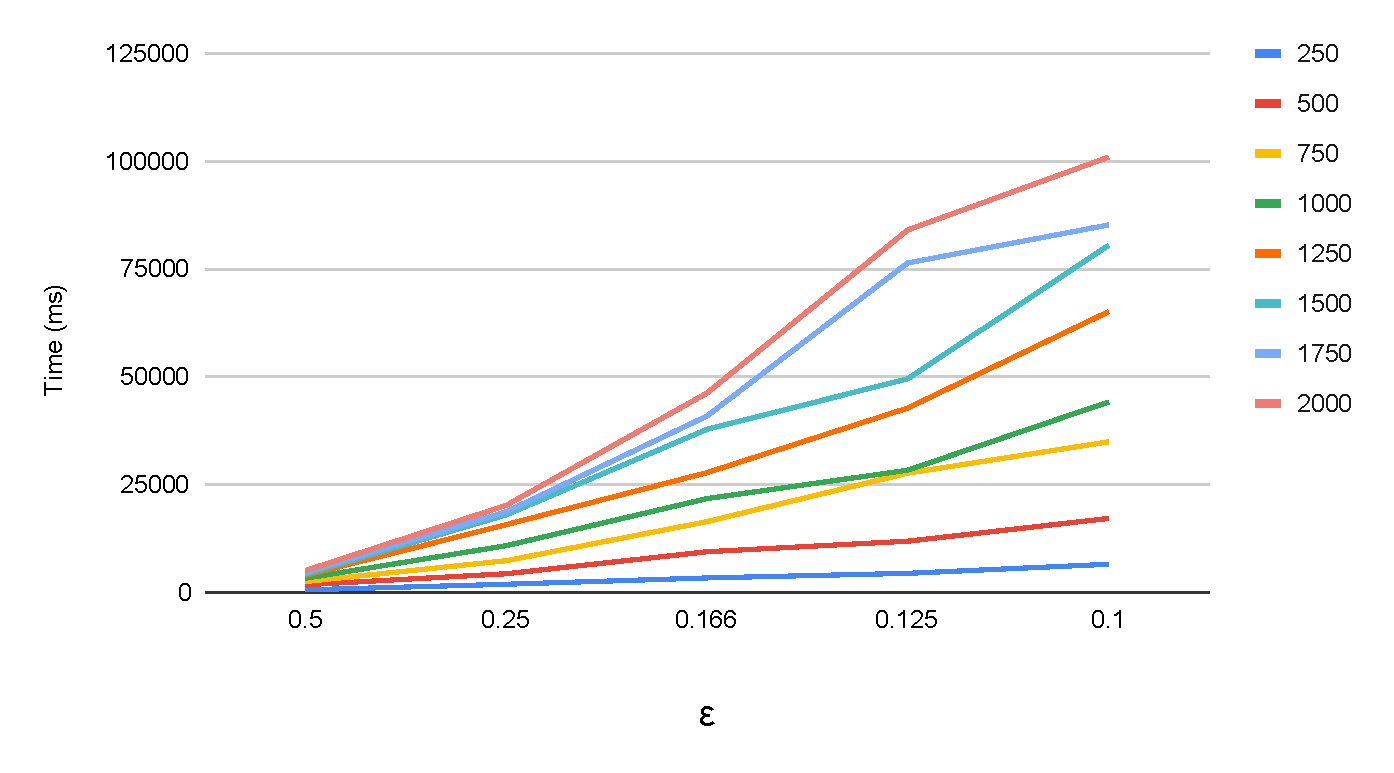
\includegraphics[width=\linewidth]{charts/epsilon.pdf}
    \caption{Running time parametrized by $\varepsilon$ for different input lengths.}
    \label{fig:chart}
\end{figure}

\begin{figure}[h!]
    \centering
    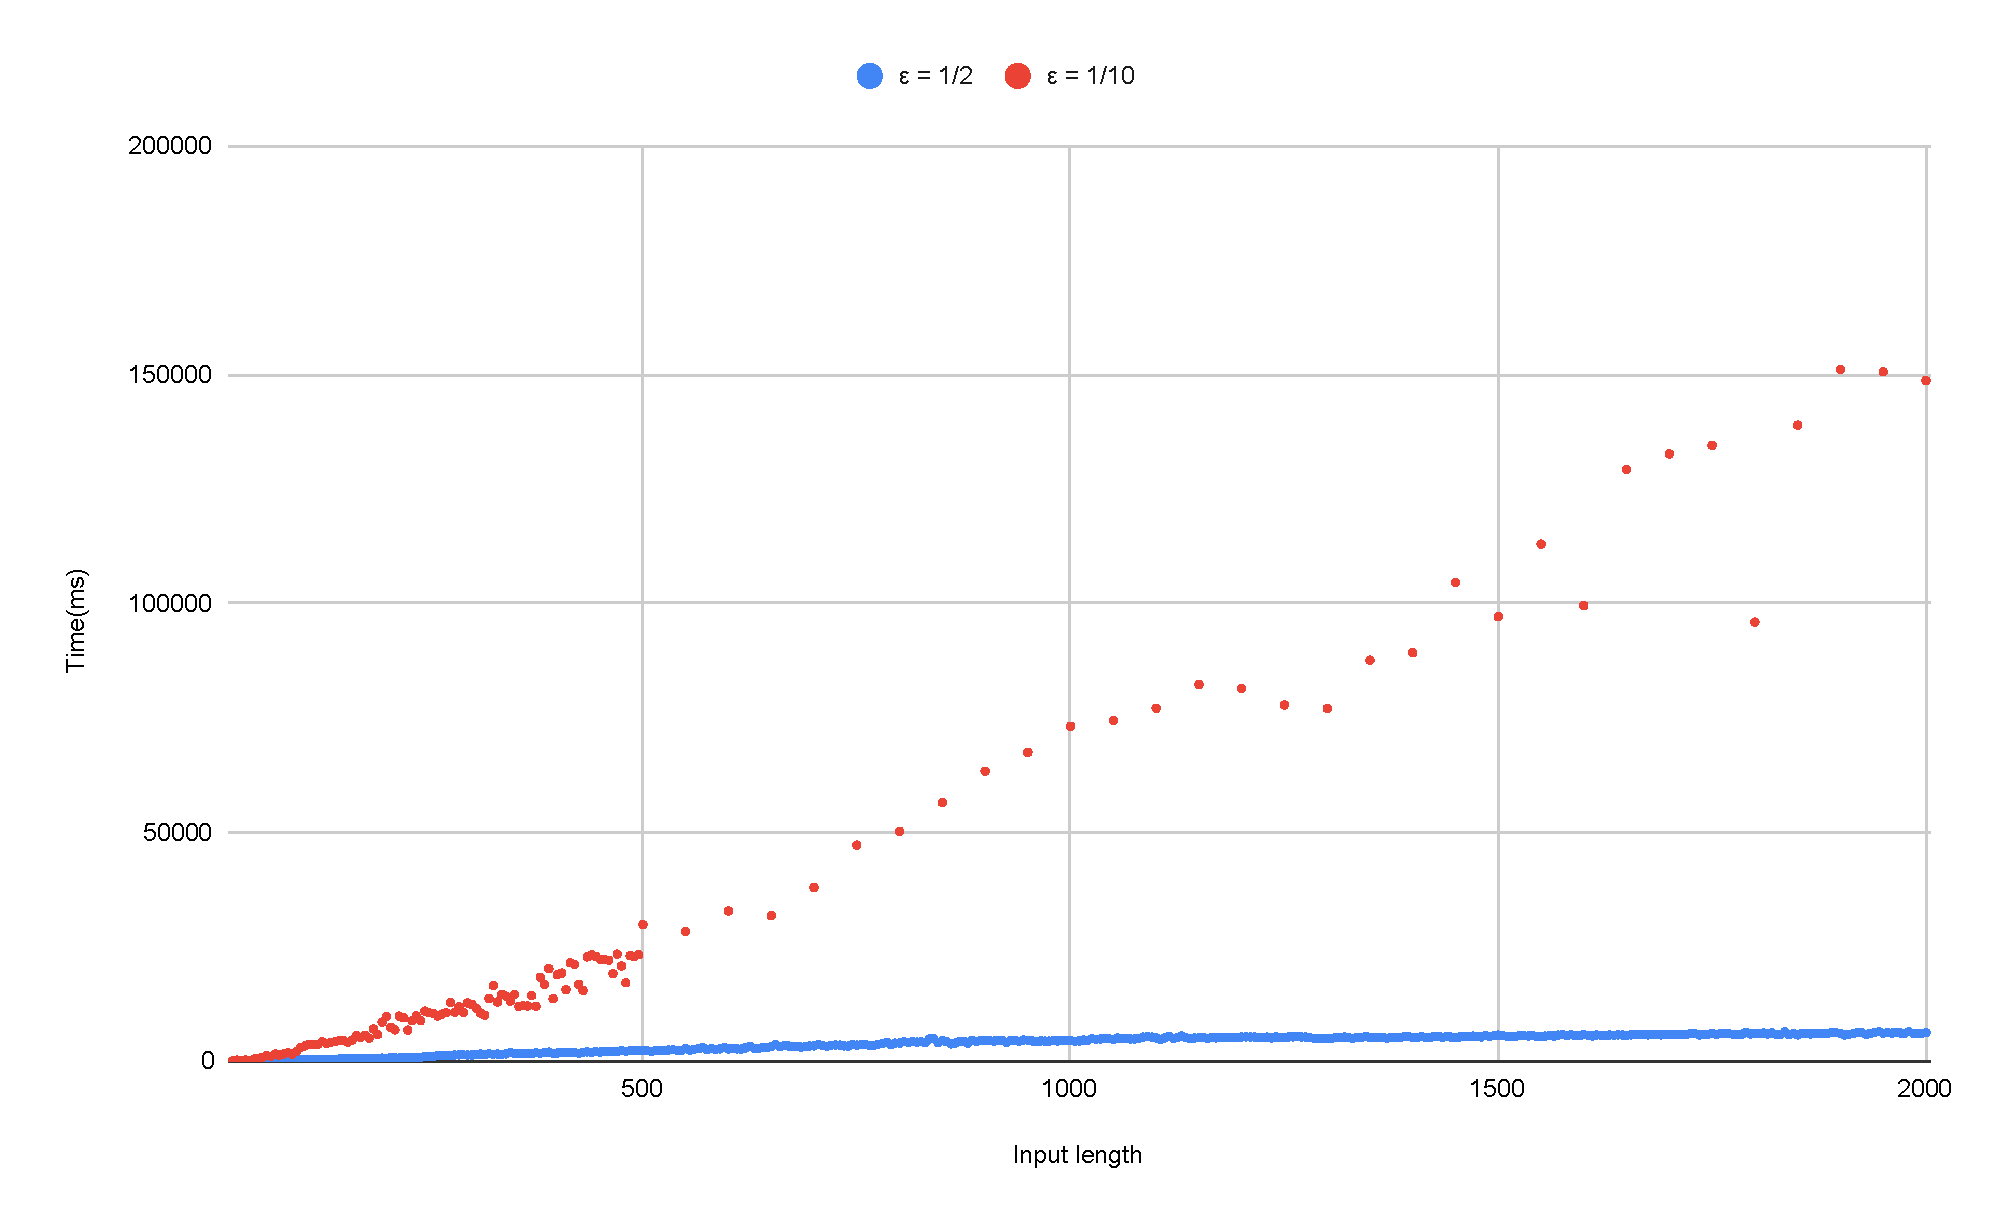
\includegraphics[width=\linewidth]{charts/input_length.pdf}
    \caption{Running time of the approximation with $\varepsilon = 1/100$ compared to a naive algorithm on a logarithmic scale.}
    \label{fig:chart}
\end{figure}

\begin{figure}[h!]
    \centering
    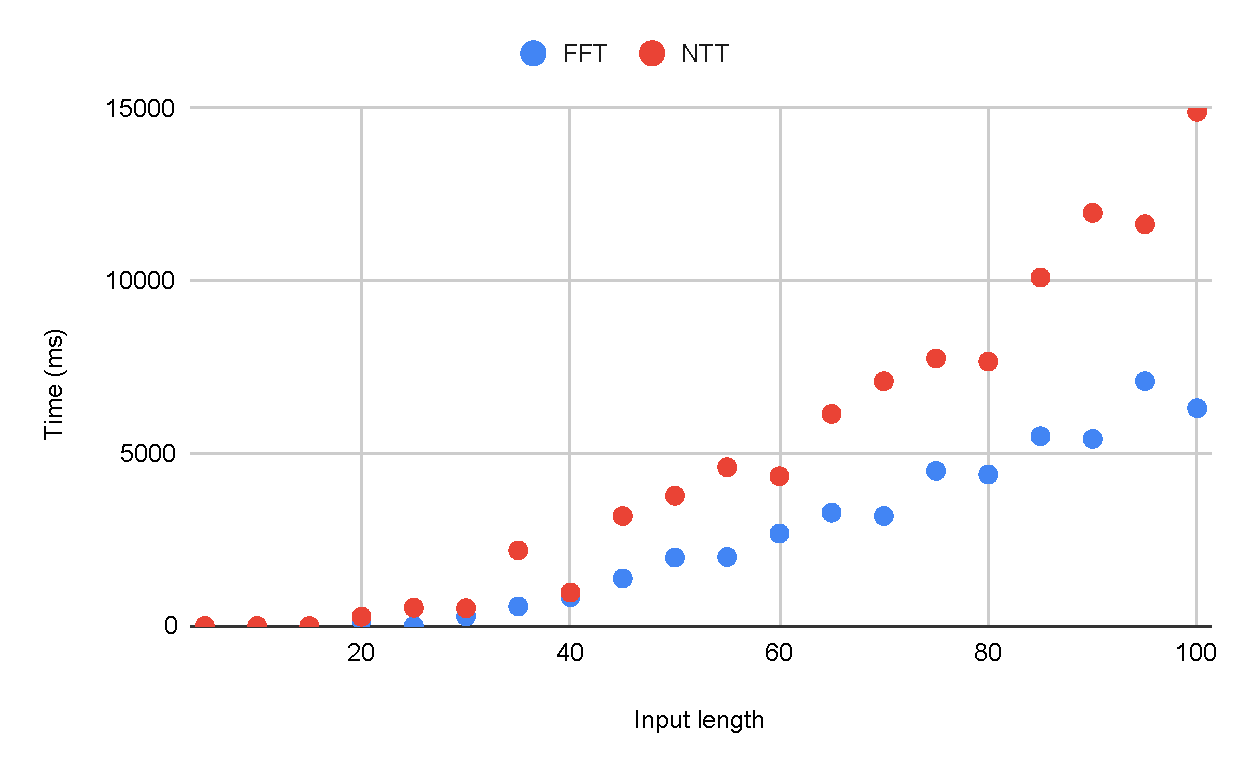
\includegraphics[width=\linewidth]{charts/fft_ntt.pdf}
    \caption{Comparison of the running time of the approximation using the FFT and NTT as convolution backends with $\varepsilon = 1/25$  }
    \label{fig:chart}
\end{figure}

\begin{figure}[h!]
    \centering
    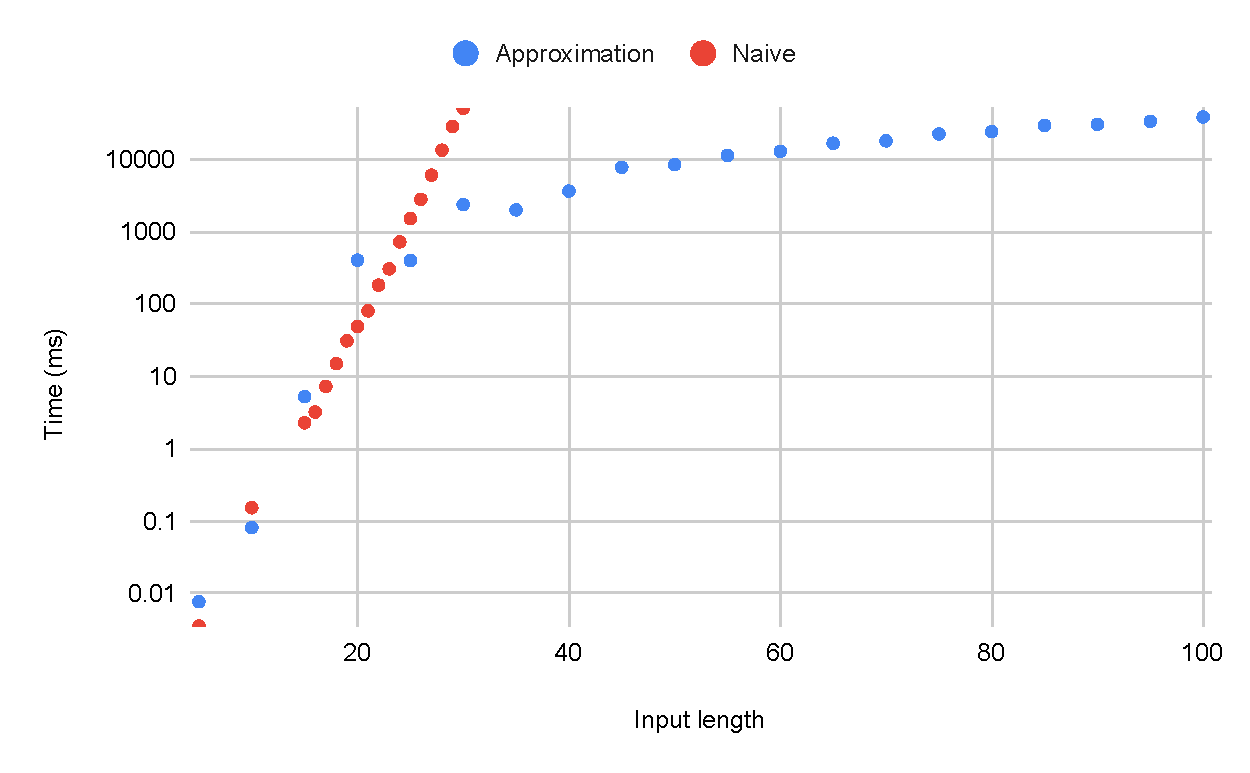
\includegraphics[width=\linewidth]{charts/naive.pdf}
    \caption{Running time of the approximation with $\varepsilon = 1/100$ compared to a naive algorithm on a logarithmic scale.}
    \label{fig:chart}
\end{figure}





\printbibliography

\end{document}
